\documentclass{../praktikum-ppt}

\author[Tew \& Haf]{Teosofi Hidayah Agung \\ Hafidz Mulia}
\date{15 Maret 2025}
\title[Alpro 2 - Week 1]{Kebenaran Algoritma}
\institute[Matematika ITS]{Departemen Matematika\\ Institut Teknologi Sepuluh Nopember}


\begin{document}

{\usebackgroundtemplate{
  \tikz[overlay,remember picture] \node[opacity=0.2, at=(current page.center)]{
\includegraphics[width=\paperwidth]{bg_22}};}
\begin{frame}
  \titlepage
\end{frame}
}

\AtBeginSection{
    {\usebackgroundtemplate{
     \tikz[overlay,remember picture] \node[opacity=0.1, at=(current page.center)]{
\includegraphics[width=\paperwidth]{code_bg}};}
    \begin{frame}{Daftar isi}
        \tableofcontents[currentsection]
        % \begin{tikzpicture}[overlay, remember picture] 
        %     \node at ([yshift=.5cm]current page.south east) [
        %         anchor = south east, 
        %         ] {
        %     \animategraphics[autoplay,loop,width=0.2\textwidth]{30}{Arisu Dance/Arisu Dance-}{0}{186}
        %     };
        % \end{tikzpicture}
    \end{frame}}
    }

    
    \begin{frame}
        \begin{masalah}
            Saat pertama kali melihat suatu kode program pastilah kita tidak akan langsung paham dengan apa yang dilakukan oleh kode tersebut. Sehingga diperlukan adanya \textbf{analisis} terhadap program apa yang dijalankan nantinya.\\

            Analisis dapat berupa apa saja, mulai dari analisa alur program, output yang dihasilkan, kompleksitas waktu dan ruang, dsb. Dalam materi kali ini kita cukup berfokus pada menganalisa kebenaran alur dan \textit{output} dari sebuah program.
        \end{masalah}
    \end{frame}

    \section{Pengertian \textit{Correctness of Algorithm}}
    \begin{frame}
      \frametitle{\insertsection}
      \begin{block}{Kebenaran Algoritma}
        \textit{\textbf{Correctness of Algorithm}} mengacu pada kepastian bahwa suatu algoritma memberikan hasil yang benar sesuai dengan spesifikasi masalah yang diberikan. Sebuah algoritma dikatakan benar (\textit{correct}), jika untuk setiap masukan yang valid, algoritma tersebut menghasilkan keluaran yang diharapkan dalam waktu yang wajar.
      \end{block}
      Analisa kebenaran algoritma cukup penting terlepas dari benar atau salah. Disisi lain analisa tersebut dapat membantu untuk menemukan sebuah solusi optimal dari suatu permasalahan.
    \end{frame}

    \begin{frame}
      \frametitle{\insertsection}
       Suatu Algoritma haruslah \textbf{efektif}, artinya:
       \begin{itemize}
        \item Algoritma harus benar dalam menyelesaikan masalah atau konteks yang diberikan.
        \item Tujuan dari pembuatannya dapat dicapai.
        \item Konsisten dalam memberikan hasil yang sama untuk masukan yang sama.
       \end{itemize}
    \end{frame}

    \begin{frame}[fragile]
      \frametitle{\insertsection}
      \begin{exampleblock}{$\,$}
      Menurut kalian apakah program berikut sudah benar sesuai intruksi yang diberikan?
      \end{exampleblock}
      \begin{columns}
        \begin{column}{0.3\textwidth}
          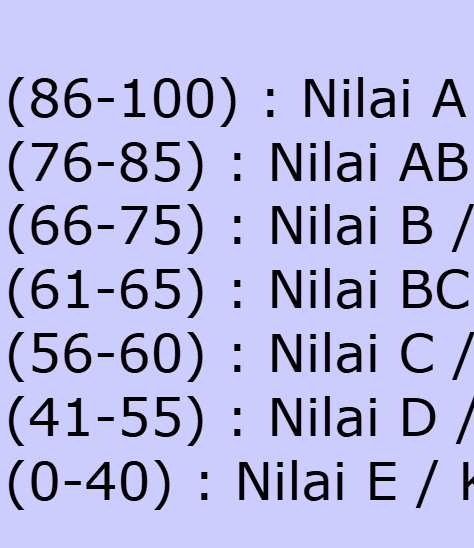
\includegraphics[width=\textwidth]{Nilai Siakad.png}
        \end{column}
        \begin{column}{0.6\textwidth}
          \begin{lstlisting}
    if (nilai >= 86 && nilai <= 100) 
      grade = "A";
    else if (nilai >= 76 && nilai <= 85) 
      grade = "AB";
    else if (nilai >= 66 && nilai <= 75) 
      grade = "B";
    else if (nilai >= 61 && nilai <= 65) 
      grade = "BC";
    else if (nilai >= 56 && nilai <= 60) 
      grade = "C";
    else if (nilai >= 41 && nilai <= 55) 
      grade = "D";
    else 
      grade = "E";
          \end{lstlisting}
        \end{column}
      \end{columns}
    \end{frame}

    \section{Tipe-tipe Kebenaran}

    \begin{frame}
      \frametitle{\insertsection}
      \textit{Correctness} dalam algoritma biasanya dikategorikan menjadi dua bagian:
      \begin{enumerate}
        \item \textbf{Partial Correctness}\\
        Berarti bahwa jika algoritma berhenti, maka hasil yang dihasilkan adalah benar. Namun, tidak menjamin bahwa algoritma akan selalu berhenti (terminate) untuk semua masukan yang valid.
        \item \textbf{Total Correctness}\\
        Sudah dipastikan bahwa algoritma tidak hanya menghasilkan hasil yang benar, tetapi juga selalu menyelesaikan eksekusinya dalam waktu yang wajar.
      \end{enumerate}
    \end{frame}

    \subsection{Partial Correctness}
    \begin{frame}[fragile]
      \frametitle{\insertsection}
      \framesubtitle{\insertsubsection}
      Kata \textbf{\textit{partial}} berarti sebagian, artinya bisa jadi terdapat suatu masukan yang dimana menghasilkan \textit{output} yang tidak benar.
      \begin{lstlisting}[caption={Nilai Maksimum Array (\textit{partial})}]
    int[] numbers = {13, 4, 24, 7};
    int maxNum = -1;
    for (int i = 0; i < numbers.length; i++) { 
        if (numbers[i] > maxNum) maxNum = numbers[i];  
    }
    System.out.println(maxNum);
      \end{lstlisting}
      \begin{exampleblock}{$\,$}
        Kira-kira apa yang salah dari program di atas?
      \end{exampleblock}
    \end{frame}

    \subsection{Total Correctness}
    \begin{frame}[fragile]
      \frametitle{\insertsection}
      \framesubtitle{\insertsubsection}
      Kata \textbf{\textit{total}} berarti keseluruhan, artinya algoritma tersebut akan selalu menghasilkan \textit{output} yang benar jika inputnya juga valid.
      \begin{lstlisting}[caption={Nilai Maksimum Array (\textit{total})}]
    int[] numbers = {13, 4, 24, 7};
    int maxNum = numbers[0];
    for (int i = 0; i < numbers.length; i++) { 
        if (numbers[i] > maxNum) maxNum = numbers[i];  
    }
    System.out.println(maxNum);
      \end{lstlisting}
      \begin{exampleblock}{$\,$}
        Bagaimana membuktikan bahwa program tersebut benar secara keseluruhan?
      \end{exampleblock}
    \end{frame}

    \begin{frame}[fragile]
      \frametitle{\insertsection}
      \begin{contoh}
        Berikut ini manakah yang termasuk dalam kategori \textit{Partial Correctness} dan \textit{Total Correctness}?
      \end{contoh}
      \begin{columns}
        \begin{column}{0.37\textwidth}
          \begin{lstlisting}[caption={Faktorial},captionpos=b]
  int factorial(int n) {
    int hasil=n;
    while(n>1){
      hasil *= n-1;
      n--;
    }
    return hasil;
  }
          \end{lstlisting}
        \end{column}
        \begin{column}{0.53\textwidth}
          \begin{lstlisting}[caption={Fibonacci},captionpos=b]
  static int fibo(int n) {
    double A = (1 + Math.sqrt(5)) / 2;
    double B = (1 - Math.sqrt(5)) / 2;
    return (int)((Math.pow(A,n) - Math.pow(B,n)) / Math.sqrt(5));
  }
          \end{lstlisting}
        \end{column}
      \end{columns}
    \end{frame}

    \section{Teknik Pembuktian}
    \begin{frame}
      \frametitle{\insertsection}
      \begin{alertblock}{Pembuktian atau Penyangkalan}
        Dalam membuktikan sesuatu yang umum, maka argumen-argumen kita harus diperumum juga. Janganlah sesekali membuktikan sebuah kebenaran di matematika menggunakan beberapa contoh kasus.

        Sebaliknya untuk menyangkal sesuatu yang umum, pakailah contoh penyangkal (\textbf{\textit{Counter Example}}) jika memang betul bahwa pernyataan tersebut salah.
      \end{alertblock}
      \begin{contoh}
        Buktikan atau sangkal pernyataan berikut:
        \begin{itemize}
          \item "$\forall x,y\in\mathbb{R}, |x+y| = |x| + |y|$"
          \item "$\forall x\forall y(xy\geq x)$"
        \end{itemize}
      \end{contoh}
    \end{frame}

    \subsection{Induksi Matematika}
    \begin{frame}
      \frametitle{\insertsection}
      \framesubtitle{\insertsubsection}
      \begin{block}{Prinsip Induksi Matematika}
        Jika kita ingin membuktikan suatu pernyataan $P(n)$ benar untuk setiap bilangan bulat $n\geq n_0$, maka kita harus membuktikan dua hal:
        \begin{enumerate}
          \item \textbf{Basis Induksi} : $P(n_0)$ benar.
          \item \textbf{Hipotesis Induksi} : Asumsikan $P(k)$ benar untuk suatu $k\geq n_0$.
          \item \textbf{Langkah Induksi} : Tunjukan bahwa $P(k+1)$ juga benar.
        \end{enumerate}
      \end{block}
      Dengan mengansumsikan $k$ adalah sebarang bilangan bulat dan jika untuk bilangan setelahnya juga benar, maka dapat disimpulkan bahwa pernyataan tersebut benar untuk setiap bilangan bulat.
    \end{frame}

    \begin{frame}[fragile]
      \frametitle{\insertsection}
      \framesubtitle{\insertsubsection}
      \begin{contoh}
        Buktikan bahwa program dibawah ini menghitung nilai $\dfrac{n(n+1)(2n+1)}{6}$
      \end{contoh}
      \begin{lstlisting}
  int sumOfSquares(int n) {
    int sum = 0;
    for (int i = 1; i <= n; i++) {
      sum += i * i;
    }
    return sum;
  }
      \end{lstlisting}
    \end{frame}

    \begin{frame}
      \frametitle{\insertsection}
      \framesubtitle{\insertsubsection}
      \begin{exampleblock}{Bukti}
        \begin{itemize}
          \item \textbf{Basis Induksi} : \onslide<2->{$P(1)$ benar, karena $1^2 = \dfrac{1(1+1)(2\cdot1+1)}{6}$}
          \item \textbf{Hipotesis Induksi} : \onslide<3->{Asumsikan $P(k):=1^2+2^2+3^2+\dots+k^2=\dfrac{k(k+1)(2k+1)}{6}$ benar untuk suatu $k\geq 1$.}
          \item \textbf{Langkah Induksi} : \onslide<4->{Akan ditunjukan bahwa $P(k+1)$ juga benar.
          \begin{flalign*}
            P(k+1):&= 1^2+2^2+\dots+k^2+(k+1)^2 = \dfrac{k(k+1)(2k+1)}{6} + (k+1)^2&\\
            &= \dfrac{k(k+1)(2k+1)+6(k+1)^2}{6} = \dfrac{(k+1)(k(2k+1)+6(k+1))}{6}&\\
            &= \dfrac{(k+1)(2k^2+7k+6)}{6}= \dfrac{(k+1)(k+2)(2k+3)}{6}\quad\square
          \end{flalign*}}
        \end{itemize}
      \end{exampleblock}
    \end{frame}

    \subsection{\textit{Loop Invariant}}
    \begin{frame}
      \frametitle{\insertsection}
      \framesubtitle{\insertsubsection}
      \begin{block}{Loop Invariant}
        \textit{Loop Invariant} adalah suatu kondisi yang selalu benar pada setiap iterasi dari suatu \textit{loop}. \textit{Loop Invariant} biasanya digunakan untuk membuktikan kebenaran dari suatu program yang menggunakan \textit{loop}.
        Terdapat tiga tahap pembuktian:
        \begin{enumerate}
          \item \textbf{Inisialisasi} : \textit{Loop Invariant} benar sebelum iterasi pertama.
          \item \textbf{Maintenance} : Jika \textit{Loop Invariant} benar sebelum iterasi ke-$k$, maka \textit{Loop Invariant} juga benar pada iterasi ke-$(k+1)$.
          \item \textbf{Terminasi} : Ketika \textit{Loop Invariant} berhenti, maka haruslah memberikan hasil yang benar sesuai spesifikasi masalah.
        \end{enumerate}
      \end{block}
    \end{frame}

    \begin{frame}[fragile]
      \frametitle{\insertsection}
      \framesubtitle{\insertsubsection}
      \begin{contoh}
        Buktikan bahwa algoritma berikut menentukan keberadaan (index) dari nilai \texttt{target} dalam sebuah array
      \end{contoh}
      \begin{lstlisting}[caption={Linear Search},captionpos=b]
  int linearSearch(int[] arr, int target) {
     for (int i = 0; i < arr.length; i++) {
         if (arr[i] == target) return i; 
     }
     return -1; 
  } 
      \end{lstlisting}
    \end{frame}

    \begin{frame}
      \frametitle{\insertsection}
      \framesubtitle{\insertsubsection}
      \begin{exampleblock}{Bukti}
        Definisikan \textit{Loop Invariant} sebagai berikut:
        \begin{quote}
          "Pada iterasi ke-\texttt{i}, semua elemen dalam array dari indeks \texttt{0} sampai \texttt{i-1} sudah diperiksa, dan jika \texttt{arr[i]==target} maka nilai telah ditemukan di indeks-\texttt{i}. Selain hal itu, target tidak ada dalam subaaray \texttt{arr[0:i-1]}."
        \end{quote}
        \vspace*{-1em}
        \begin{enumerate}
          \item \textbf{Inisialisasi} : \onslide<2->{Sebelum loop dijalankan (\texttt{i = 0}), belum ada elemen yang diperiksa. Pernyataan \textit{loop invariant} tetap benar karena tidak ada elemen yang diperiksa sebelum iterasi pertama.}
          \item \textbf{Maintenance} : \onslide<3->{Pada iterasi ke-\texttt{i},  kita mengecek elemen \texttt{arr[i]}:
          \begin{itemize}
            \item Jika \texttt{arr[i] == target}, maka kita mengembalikan \texttt{i}, yang berarti target ditemukan.
            \item Jika tidak, kita lanjut ke elemen berikutnya.
          \end{itemize}
          \textit{Loop invariant} tetap benar karena elemen sebelum indeks \texttt{i+1} telah diperiksa.
          }
        \end{enumerate}
      \end{exampleblock}
    \end{frame}

    \begin{frame}
      \frametitle{\insertsection}
      \framesubtitle{\insertsubsection}
      \begin{exampleblock}{Bukti (lanj.)}
        \begin{enumerate}
          \setcounter{enumi}{2}
          \item \textbf{Terminasi} : \onslide<2->{Ketika loop berhenti, ada dua kemungkinan:
          \begin{itemize}
            \item Jika \texttt{target} ditemukan, maka kita mengembalikan indeksnya.
            \item Jika tidak, maka kita mengembalikan -1, yang berarti \texttt{target} tidak ada dalam array.
          \end{itemize}
          Kedua kasus tersebut sesuai dengan spesifikasi masalah.}
        \end{enumerate}
        \onslide<3->{Jadi algoritma tersebut benar dalam menentukan keberadaan/indeks \texttt{target} dalam array.}
      \end{exampleblock}
    \end{frame}

    \subsection{Metode Formal}
    \begin{frame}
      \frametitle{\insertsection}
      \framesubtitle{\insertsubsection}
      \begin{block}{Metode Formal}
        Metode formal adalah teknik pembuktian kebenaran algoritma yang menggunakan logika matematika. Metode ini biasanya digunakan untuk membuktikan kebenaran algoritma yang kompleks. Ada dua kunci dalam pembuktian ini, antara lain:
        \begin{enumerate}
          \item \textbf{Preconditions}: Keadaan yang harus benar \underline{sebelum} algoritma dijalankan.
          \item \textbf{Postconditions}: Keadaan yang harus benar \underline{setelah} algoritma dijalankan.
        \end{enumerate}
      \end{block}
    \end{frame}

    \begin{frame}[fragile]
      \frametitle{\insertsection}
      \framesubtitle{\insertsubsection}
      \begin{contoh}
        Buktikan bahwa program dibawah ini menghitung nilai $x^n$ dengan $n$ bulat non-negatif.
      \end{contoh}
      \begin{lstlisting}
    public static double power(double x, int n) {
      if (n == 0) {
          return 1;
      }
      double half = power(x, n / 2);
      if (n % 2 == 0) {
          return half * half; 
      } else {
          return x * half * half; 
      }
    }
      \end{lstlisting}
    \end{frame}

    \begin{frame}
      \frametitle{\insertsection}
      \framesubtitle{\insertsubsection}
      \begin{exampleblock}{Bukti}
        \begin{enumerate}
          \item \textbf{Preconditions} : 
          \onslide<2->{\begin{itemize}
            \item $x$ bisa berupa bilangan real (termasuk negatif dan pecahan).
            \item $n$ adalah bilangan bulat non-negatif.
          \end{itemize}
          Jika $n$ negatif, maka algoritma tidak valid karena tidak menangani eksponen negatif.
          }
          \item \textbf{Postconditions} : \onslide<3->{$\text{power}(x,n)=x^n$
          \begin{itemize}
            \item Basis $n=0$ berakibat $x^0=1$.
            \item Jika $n$ genap, maka $x^n=(x^{n/2})^2$.
            \item Jika $n$ ganjil, maka $x^n=x\cdot(x^{n/2})^2$.
          \end{itemize}
          }
        \end{enumerate}
        \onslide<4->{Dengan menggunakan metode formal, kita dapat membuktikan bahwa program tersebut benar dalam menghitung nilai $x^n$ dengan $n\in\mathbb{N}\cup{0}$.}
      \end{exampleblock}
    \end{frame}

    \begin{frame}
      \frametitle{\insertsection}
      \begin{table}
        \centering \scriptsize
        \caption{Perbandingan Metode Pembuktian Kebenaran Algoritma}
        \begin{tabular}{|>{\columncolor{HIMAabu}}m{2.1cm}|m{3.8cm}|m{3.3cm}|m{3cm}|}
          \hline
          \textbf{Metode} & \textbf{Fokus} & \textbf{Cakupan} & \textbf{Contoh Algoritma} \\
          \hline
          \textbf{Induksi \textcolor{HIMAabu}{....} Matematika} & Untuk membuktikan kebenaran rumus matematika atau algoritma rekursif & Algoritma berbasis \underline{rekursi} atau \underline{perulangan} yang memiliki \underline{pola matematis} & Faktorial, Fibonacci, jumlah deret, Hanoi Tower \\
          \hline
          \textbf{Loop Invariant} & Untuk membuktikan algoritma berbasis perulangan agar tetap mempertahankan sifat tertentu selama eksekusi & Algoritma yang menggunakan \underline{loop (iteratif)} & \textit{sorting} dan \textit{searching} \\
          \hline
          \textbf{Pembuktian Formal} & Untuk membuktikan keabsahan algoritma secara umum tanpa harus bergantung pada perulangan atau rekursi. & Memberikan \underline{bukti formal untuk} \underline{keseluruhan algoritma}, termasuk rekursi, loop, dan kondisi lainnya. &  Euclidean GCD, Exponentiation by Squaring, Divide and Conquer, Dynamic Programming \\
          \hline
      \end{tabular}
      \end{table}
    \end{frame}

    \section{Latihan}
    \begin{frame}[fragile]
      \begin{latihan}
        Buktikan bahwa fungsi berikut menghitung jumlahan digit suatu bilangan bulat
      \end{latihan}
      \begin{lstlisting}
  int jumlahDigit(int X) {
    if (X == 0) return 0;
    else return (X % 10) + jumlahDigit(X / 10);
  }
      \end{lstlisting}
      \begin{latihan}
        Telusuri fungsi berikut dan buktikan kebenaran dari fungsi tersebut.
      \end{latihan}
      \begin{lstlisting}
  boolean cek(string S) {
    for (int i = 0; i < n-1; i++) {
      if (S[i] > S[i+1]) return false;
      } 
    return true;
  } 
      \end{lstlisting}
    \end{frame}
\end{document}
